\chapter{Medidas de avaliação de qualidade}
\label{chapter:metrics}

O mérito geral de um método de estimação depende de muitos fatores: sua complexidade
computacional e as condições pressupostas pela solução são dois exemplos evidentes.
Embora importantes --- características como essas serão inevitavelmente discutidas nas
análises dos modelos ---, este trabalho dará destaque especial à que seja provavelmente
a qualidade-mor de um método: sua eficácia em estimar o sinal desejado. Para tanto,
precisamos considerar a fidelidade da estimação quando comparada à gravação distorcida
isolada.

Para avaliar a qualidade de uma gravação sonora, podemos fazer testes subjetivos ou
objetivos. No primeiro caso, participantes dão notas aos sinais avaliados considerando
um sinal de referência. Este processo é complexo e facilmente suscetível a erros, pois
precisamos de uma boa amostra de voluntários e equipamentos adequados. Nos testes
objetivos, utilizamos equações e algoritmos prontos para calcular as ``notas'' (que
podem ser de fato valores dentro de intervalos pré-definidos, ou medidas mais
abrangentes), não dependendo do fator humano.

Pela simplicidade dos métodos objetivos (se comparados aos subjetivos), estes foram
escolhidos para serem utilizados na pesquisa. Mais especificamente, serão consideradas
três medidas: a \textit{Source-to-Distortion Ratio}
(SDR)\abbrev{SDR}{\textit{Source-to-Distortion Ratio}}~\cite{vincent-2006}, que
quantifica a presença de distorção no sinal estimado; a \textit{Perceptual Audio
	Quality Measure} (PAQM)\abbrev{PAQM}{\textit{Perceptual Audio Quality
		Measure}}~\cite{beerends-1992}, que gradua a qualidade da estimação usando uma
modelagem psicoacústica; e a \rnonlin{}~\cite{tan-2004}, que também considera a
Psicoacústica para avaliar a existência de distorções não-lineares em um sinal
processado.

\section{\textit{Source-to-Distortion Ratio} (SDR)}
\label{section:metrics:sdr}

A \textit{Source-to-Distortion Ratio} foi originalmente proposta, junto a outras três
medidas, como um indicador de desempenho para algoritmos de separação cega de fontes
sonoras~\cite{vincent-2006}. Por questões de completude, iremos agora apresentar todas
essas medidas, e não só a SDR, embora apenas esta seja utilizada no trabalho.

Pressuponha que, a partir de uma mistura de fontes e utilizando um algoritmo de
separação de fontes sonoras, gerou-se a estimação $\hat{d}_j[n]$ do sinal $d_j[n]$
proveniente da fonte $j$. Este sinal pode ser decomposto em quatro componentes:
\begin{equation}
	\hat{d}_j[n] = d_j[n] + e_{\text{interf}}[n] + e_{\text{ruído}}[n] + e_{\text{artef}}[n].
	\label{eq:metrics:d-hat}
\end{equation}

O primeiro componente é o sinal que se deseja segregar da mistura.\footnote{Este pode
ser uma versão de um sinal original $x_j[n]$, com distorções ``aceitas'' pelo
algoritmo; é o caso deste trabalho, em que elas são não só possíveis como desejadas.}
Idealmente, $\hat{d}_j[n] = d_j[n]$; porém, durante o processo de separação, sinais
espúrios podem aparecer na estimação resultante. Tais sinais indesejados podem ser
classificados em três tipos: interferência por outras fontes, ruído (oriundo de fontes
não consideradas na separação) e artefatos introduzidos pelo algoritmo.

Sendo $\Vert s \Vert^2$\symbl{$\Vert \cdot \Vert$}{Norma euclidiana} a energia total de
uma sequência finita $s[n]$, definem-se as seguintes medidas de qualidade, todas
expressas em decibéis: a \textit{Source-to-Distortion Ratio},
\begin{equation}
	\text{SDR} \coloneqq 10 \log_{10} \frac{\Vert d_j \Vert^2}{\Vert e_{\text{interf}} + e_{\text{ruído}} + e_{\text{artef}} \Vert^2};
	\label{eq:metrics:sdr-original}
\end{equation}
a \textit{Source-to-Interference Ratio}\abbrev{SIR}{\textit{Source-to-Interference Ratio}},
\begin{equation}
	\text{SIR} \coloneqq 10 \log_{10} \frac{\Vert d_j \Vert^2}{\Vert e_{\text{interf}} \Vert^2};
\end{equation}
a \textit{Sources-to-Noise Ratio}\abbrev{SNR}{\textit{Sources-to-Noise Ratio}},
\begin{equation}
	\text{SNR} \coloneqq 10 \log_{10} \frac{\Vert d_j + e_{\text{interf}} \Vert^2}{\Vert e_{\text{ruído}}\Vert^2};
\end{equation}
e a \textit{Sources-to-Artifacts Ratio}\abbrev{SAR}{\textit{Sources-to-Artifacts Ratio}},
\begin{equation}
	\text{SAR} \coloneqq 10 \log_{10} \frac{\Vert d_j + e_{\text{interf}} + e_{\text{ruído}}\Vert^2}{\Vert e_{\text{artef}} \Vert^2}.
\end{equation}

Usando a relação da Equação~\eqref{eq:metrics:d-hat} e abstraindo-nos do fato de que
estamos avaliando a qualidade da $j$-ésima fonte, é possível reescrever a
Equação~\eqref{eq:metrics:sdr-original} como
\begin{equation}
	\text{SDR} = 10 \log_{10} \frac{\Vert d \Vert^2}{\Vert \hat{d} - d \Vert^2}.
	\label{eq:metrics:sdr}
\end{equation}

Analisando a Equação~\eqref{eq:metrics:sdr}, pode-se concluir que, mesmo em cenários
mais amplos, a SDR é uma medida adequada para mensurar a semelhança entre um sinal
desejado (e conhecido) $d[n]$ e sua estimação $\hat{d}[n]$. Assim, quanto maior o valor
da SDR, mais numericamente semelhantes são duas gravações.

\section{\textit{Perceptual Audio Quality Measure} (PAQM)}
\label{section:metrics:paqm}

Embora suficientemente poderosa, a SDR avalia apenas a diferença absoluta entre dois
sinais, sem nenhuma consideração contextual. Para suprir essa ausência, surgem os
modelos psicoacústicos: na comparação entre gravações sonoras, se pressupusermos que o
receptor final será o ouvido humano, podemos levar em conta as particularidades do
sistema auditivo na hora de determinar a qualidade de um sinal. Em outras palavras,
metrifica-se a semelhança percebida, não a absoluta.

Os métodos psicoacústicos estão intimamente relacionados a testes subjetivos; afinal, é
considerando as opiniões de ouvintes reais que podemos validar um sistema computacional
equivalente. Nestes testes~\cite{bech-2006}, os participantes devem avaliar a qualidade
de uma gravação a partir de um áudio de referência, assim como nos algoritmos
objetivos. Uma medida muito utilizada nesses experimentos é a \textit{Mean Opinion
	Score} (MOS)\abbrev{MOS}{\textit{Mean Opinion Score}}, que é a média entre as notas
individuais de cada participante; nas definições usuais, seu valor varia de 1 (péssimo)
a 5 (excelente).

A \textit{Perceptual Audio Quality Measure} (PAQM)~\cite{beerends-1992} é uma medida
que visa a avaliar comparativamente a qualidade de uma gravação considerando as
particularidades psicoacústicas mencionadas. Para isso, o algoritmo transforma as duas
gravações (o sinal de referência e o avaliado) em suas respectivas ``representações
internas'' --- aproximações de como os sinais são percebidos pelo nosso sistema
auditivo ---, e metrifica a diferença entre elas. São várias as etapas características
da audição humana a serem modeladas pelo sistema: i) na orelha externa, a pina
(pavilhão auricular) filtra e concentra o som, que passa então pelo canal auditivo; ii)
a orelha média transfere as vibrações do ar para iii) a orelha interna, na qual se
tornam vibrações num líquido e se originam efeitos psicoacústicos como espalhamento,
compressão, e mascaramento. Antes de discutirmos o algoritmo em si, vamos nos debruçar
rapidamente sobre esses efeitos.

O mascaramento é o mais importante dos fenômenos mencionados. O efeito ocorre quando
certos tons na gravação se tornam inaudíveis devido a outros componentes de maior
intensidade que estejam próximos no tempo e/ou na frequência. Imagine, por exemplo, a
dificuldade que seria de se ouvir a queda de uma agulha se um revólver fosse disparado
ao mesmo tempo: este é um exemplo trivial (e radical) de mascaramento. Cada componente
tempo-frequencial de um sinal possui uma \emph{curva de mascaramento} associada, e
essas curvas se combinam para formar um limiar de audibilidade: qualquer tom abaixo
desse limiar é considerado inaudível.

As curvas de mascaramento, porém, não são apenas cópias exatas dos perfis dos
componentes tempo-frequenciais. Para gerá-las, é preciso considerar os outros dois
efeitos mencionados anteriormente. O primeiro é o espalhamento, que caracteriza o fato
de que a curva associada a um tom ``se espalha'' para além dele próprio, tanto no tempo
quanto na frequência; deste modo, componentes vizinhos aos tons mais intensos, mas não
totalmente sobrepostos, podem ser mascarados. Já a compressão emula nossa sensibilidade
auditiva não-linear para intensidade: nossos ouvidos são mais sensíveis a sons (e
variações) menos intensos, e, quanto maior a intensidade absoluta, menor a variação
percebida. Assim, as curvas são calculadas de acordo com a intensidade percebida de
cada componente. A Figura~\ref{fig:metrics:masking} ilustra um exemplo de curvas de
mascaramento para um tom senoidal de curta duração.
\begin{figure}[!ht]
	\centering
	\begin{subfigure}[t]{\textwidth}
		\centering
		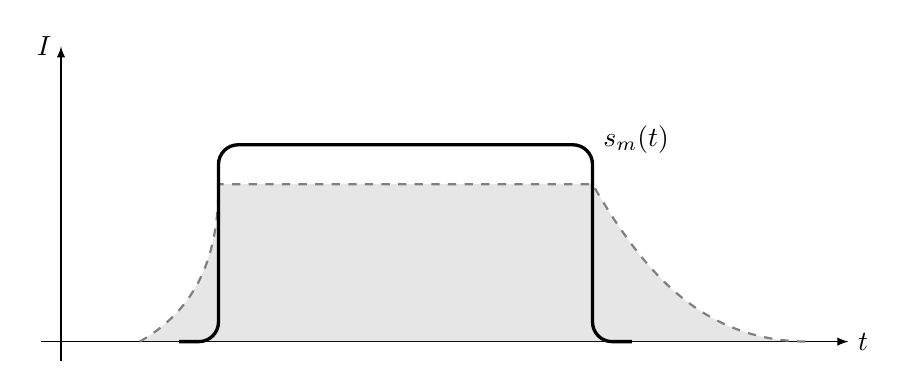
\begin{tikzpicture}
    \draw[-latex] (-0.25, 0) -- (10, 0) node[right] {$t$};
    \draw[-latex] (0, -0.25) -- (0, 3.75) node[left] {$I$};

    % Masker tone
    \begin{scope}[shift={(0.5, 0)}]
        \begin{scope}[shift={(0,0)}]
            \filldraw[dashed, thick, gray, fill opacity=0.2] (0.5, 0) to[out=30, in=-90] (1.5, 2) -- (6.25, 2) to[out=-60, in=180] (9, 0);
        \end{scope}
        \draw[very thick] (1, 0) -- (1.25, 0) to[out=0, in=-90] (1.5, 0.25) -- (1.5, 2.25) to[out=90, in=180] (1.75, 2.5) -- (6, 2.5) to[out=0, in=90] (6.25, 2.25) node[above right] {$s_m(t)$} -- (6.25, 0.25) to[out=-90, in=180] (6.5, 0) -- (6.75, 0);
    \end{scope}
\end{tikzpicture}

		\caption{Caso temporal.}
		\label{fig:metrics:time-masking}
	\end{subfigure}

	\medskip

	\begin{subfigure}[t]{\textwidth}
		\centering
		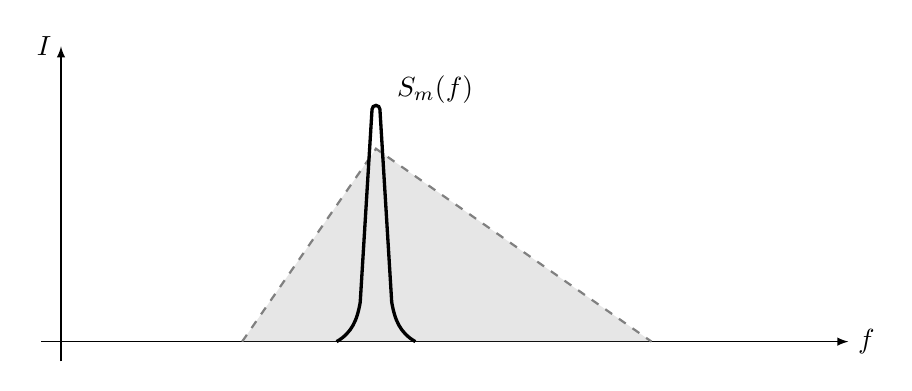
\begin{tikzpicture}
    \draw[-latex] (-0.25, 0) -- (10, 0) node[right] {$f$};
    \draw[-latex] (0, -0.25) -- (0, 3.75) node[left] {$I$};

    % Masker tone
    \begin{scope}[shift={(1,0)}]
    \filldraw[dashed, thick, gray, fill opacity=0.2] (1.3, 0) -- (3, 2.45) -- (6.5, 0);
    \draw[very thick] (2.5, 0) to[out=30, in=-100] (2.8, 0.5) -- (2.95, 2.95) arc (180:0:0.05) -- (3.2, 0.5) to[out=-80, in=150] (3.5, 0);
    \draw (3.75, 3.2) node[] {$S_m(f)$};
    \end{scope}

    % Masked tone
    %\draw[very thick, -latex] (5, 0) node[below] {$f_2$} -- (5, 0.75) node[left] {$s_2(t)$};
\end{tikzpicture}

		\caption{Caso frequencial.}
		\label{fig:metrics:frequency-masking}
	\end{subfigure}

	\caption[Exemplos de curvas de mascaramento no tempo e na frequência]{Exemplos de curvas de mascaramento (linhas tracejadas) no tempo e na frequência para um tom senoidal contínuo $s_m(t)$ de curta duração. As curvas cheias representam a intensidade do sinal, não a senoide em si. Note que as curvas ``se espalham'' ao redor do tom, resultado do efeito de espalhamento. Como estamos representando apenas um componente, o fenômeno de compressão não foi ilustrado. A curva de mascaramento final é a combinação das curvas dos dois domínios; qualquer tom abaixo dessa curva (dentro da hachura) é considerado inaudível.}
	\label{fig:metrics:masking}
\end{figure}

Podemos agora apresentar o método. Embora originalmente proposto
em~\cite{beerends-1992}, focaremos na descrição presente em~\cite{beerends-2002}, porém
com duas importantes adaptações. No texto consultado, o algoritmo foi descrito para o
domínio contínuo; como todo este trabalho é baseado em processamentos digitais, as
definições e funções foram modificadas para manter esta consistência. Além disso,
usaremos $d[n]$ e $\hat{d}[n]$ para representar o sinal de referência e o avaliado,
respectivamente --- em vez de $x[n]$ e $y[n]$ do texto base ---, também para seguir as
convenções do projeto. Os passos para o cálculo da medida são então (ver
Figura~\ref{fig:metricas:paqm-diagram} para uma diagrama do algoritmo):
\begin{enumerate}
	\item O sinal de referência $d[n]$ e o sinal a ser avaliado $\hat{d}[n]$ são transformados
	      para o domínio tempo-frequencial usando um janela de Hann de 40~ms (logo, é preciso
	      saber a frequência de amostragem $f_s$\symbl{$f_s$}{Frequência de amostragem das
		      gravações sonoras}), resultando nos espectrogramas de potência $P_d[m, k]$ e
	      $P_{\hat{d}}[m, k]$, em que $m$ indexa os segmentos temporais e $k$ indexa os
	      \textit{bins} frequenciais. Isto é feito pois, como vimos, os fenômenos são modelados
	      por métodos tempo-frequenciais. Ademais, o processamento em blocos leva em consideração
	      a não-estacionariedade usual em sinais de áudio.

	\item A escala frequencial $k$ (em \textit{bins} igualmente espaçados em hertz) é convertida
	      para uma escala de \textit{pitch} $z$ (em \textit{bins} igualmente espaçados em barks).
	      A escala Bark modifica a escala de frequência original em Hz para ficar proporcional à
	      resolução frequencial da audição humana. Então, ambos os sinais são filtrados por uma
	      resposta na frequência $a_0[z]$ que engloba todo o processamento linear feito pelo
	      sistema auditivo, resultando em $p_d[m, z]$ e $p_{\hat{d}}[m, z]$.

	\item Cada bloco de $p_d[m, z]$ e $p_{\hat{d}}[m, z]$ é combinado, na norma
	      $\alpha_{\text{temp}}$,\footnote{A combinação de valores em uma norma $\alpha$ é
		      definida por $(\sum_i x_i^\alpha)^{\frac{1}{\alpha}}$.} com o bloco temporal anterior
	      multiplicado por uma função $e^{h(m, z)}$. Esta etapa é responsável por modelar o
	      espalhamento temporal, e depende do tamanho do salto entre dois janelamentos
	      consecutivos.

	\item As representações são individualmente convoluídas com uma função de espalhamento
	      frequencial. Este processo é não-linear, pois as curvas de espalhamento de diferentes
	      \textit{bins} são combinadas na norma $\alpha_{\text{freq}}$. Com os espalhamentos no
	      tempo e na frequência modelados, encontramos as representações $E_d[m, z]$ e
	      $E_{\hat{d}}[m, z]$.

	\item O efeito de compressão é aplicado individualmente nas representações $E_d[m, z]$ e
	      $E_{\hat{d}}[m, z]$, que se tornam $\mathcal{L}_d[m, z]$ e $\mathcal{L}_{\hat{d}}[m,
		      z]$. O algoritmo de compressão aplicado depende do hiperparâmetro $\gamma$, um
	      parâmetro de compressão ajustável.

	\item A representação $\mathcal{L}_{\hat{d}}[m, z]$ recebe uma correção de ganho em
	      diferentes faixas de \textit{pitch}. Esta etapa é responsável por uma ``correspondência
	      de padrões'' (\textit{pattern matching}) entre as duas representações, e engloba outras
	      etapas do processo psicoacústico não contempladas explicitamente pelo algoritmo.

	\item Calcula-se a diferença absoluta entre $\mathcal{L}_d[m, z]$ e
	      $\mathcal{L}_{\hat{d}}'[m, z]$ (pós-ganho), resultando na função de densidade de
	      perturbação de ruído $\mathcal{L}_n[m, z]$. Todos os valores dos \textit{bins}
	      frequenciais para um bloco $k$ são somados, e então a média entre os blocos é
	      calculada; assim, encontramos a perturbação de ruído
	      $\mathcal{L}_n$\symbl{$\mathcal{L}_n$}{Perturbação de ruído calculado pela PAQM}.
	      Finalmente, a PAQM é definida como sendo $\log_{10}(\mathcal{L}_n)$.
\end{enumerate}

\begin{figure}[hbtp]
	\centering
	\tikzset{
    compression-func/.pic={
        \begin{scope}[shift={(-0.9, -0.5)}]
            \draw[-latex] (-0.1, 0) -- (1.75, 0) node[above] {\scriptsize$E$};
            \draw[-latex] (0, -0.1) -- (0, 1) node[right] {\scriptsize$\mathcal{L}$};
            \draw[thick] (0.25, 0) to[out=80, in=-170] (1.65, 0.9);
        \end{scope}
    },
    freqspread-func/.pic={
        \begin{scope}[shift={(-0.9, -0.5)}]
            \draw (0, 0) -- (1.8, 0);
            \filldraw[dashed, thick, gray, fill opacity=0.2] (0.45, 0) -- (0.6, 0.9) -- (1.4, 0);
        \end{scope}
    },
    linearfilter/.pic={
        \begin{scope}[shift={(-0.9, -0.5)}]
            \draw[-latex] (-0.1, 0) -- (1.75, 0) node[above] {\scriptsize$z$};
            \draw[-latex] (0, -0.1) -- (0, 1) node[right] {\scriptsize$a_0$};
            \draw[thick] (0, 0) to[out=60, in=180] (0.5, 0.6) -- (0.8, 0.55) to[out=0, in=180] (1.1, 0.7) to[out=0] (1.5, 0);
        \end{scope}
    },
    freqconversion-func/.pic={
        \begin{scope}[shift={(-0.9, -0.5)}]
            \draw[-latex] (-0.1, 0) -- (1.75, 0) node[above] {\scriptsize$k$};
            \draw[-latex] (0, -0.1) -- (0, 1) node[right] {\scriptsize$z$};
            \draw[thick] (0, 0) to[out=60, in=-170] (1.6, 1);
        \end{scope}
    },
    window/.pic={
        \draw[thick] (-0.9, -0.375) sin (0, 0.375);
        \draw[thick] (0, 0.375) cos (0.9, -0.375);
    }
}

\begin{tikzpicture}[node distance=0.9cm and 2.5cm]
    % Drawing from bottom to top for easier organization
    \node[coordinate] (paqm) {};

    \node[dspfilter, above=of paqm, minimum height=1cm] (log10) {$\log_{10}(\cdot)$};
    \draw[dspconn] (log10) -- node[midway,left] {PAQM} (paqm);

    \node[dspfilter, left=of log10, minimum height=1cm, xshift=0.75cm] (time-freq-mean) {$\frac{1}{N}\sum_m\sum_z$};
    \draw[dspconn] (time-freq-mean) -- node[midway,above] {$\mathcal{L}_n$} (log10);
    
    %\node[below=of paqm, yshift=0.5cm] (whitespace) {};

    \node[dspfilter, left=of time-freq-mean, minimum height=1cm, xshift=0.75cm] (abs) {$|\cdot|$};
    \draw[dspconn] (abs) -- node[midway,above] {$\mathcal{L}_n[m, z]$} (time-freq-mean);

    \node[dspadder, above=of abs, yshift=-0.25cm] (diff) {};
    \draw[dspconn] (diff) -- (abs);

    %%%%%%%%%%% DHAT
    \node[dspfilter, above right=of diff, minimum height=1cm, yshift=-0.65cm] (scaling) {Ganho};
    \draw[dspconn] (scaling) |- node[midway,right] {$\mathcal{L}'_{\hat{d}}[m, z]$} (diff);
    \node[xshift=0.65cm, yshift=0.3cm] (plus) at (diff) {$+$};

    \node[dspfilter, minimum height=1.5cm, above=of scaling] (compression-dhat) {};
    \pic[] at (compression-dhat) {compression-func};
    \draw[dspconn] (compression-dhat) -- node[midway,right] {$\mathcal{L}_{\hat{d}}[m, z]$} (scaling);

    \node[dspfilter, minimum height=1.5cm, above=of compression-dhat] (freqspread-dhat) {};
    \pic[] at (freqspread-dhat) {freqspread-func};
    \draw[dspconn] (freqspread-dhat) -- node[midway,right] {$E_{\hat{d}}[m, z]$} (compression-dhat);

    \node[dspfilter, above=of freqspread-dhat, minimum height=1cm] (timespread-dhat) {$+$, $e^{h(m, z)}$};
    \draw[dspconn] (timespread-dhat) -- (freqspread-dhat);

    \node[dspfilter, minimum height=1.5cm, above=of timespread-dhat] (linearfilter-dhat) {};
    \pic[] at (linearfilter-dhat) {linearfilter};
    \draw[dspconn] (linearfilter-dhat) -- node[midway,right] {$p_{\hat{d}}[m, z]$} (timespread-dhat);
    
    \node[dspfilter, minimum height=1.5cm, above=of linearfilter-dhat] (freqconversion-dhat) {};
    \pic[] at (freqconversion-dhat) {freqconversion-func};
    \draw[dspconn] (freqconversion-dhat) -- node[midway,right] {$P_{\hat{d}}[m, z]$} (linearfilter-dhat);

    \node[dspfilter, above=of freqconversion-dhat, minimum height=1cm] (density-dhat) {$|\cdot|^2$};
    \draw[dspconn] (density-dhat) -- node[midway,right] {$P_{\hat{d}}[m, k]$} (freqconversion-dhat);

    \node[dspfilter, above=of density-dhat, minimum height=1cm] (fft-dhat) {FFT};
    \draw[dspconn] (fft-dhat) -- (density-dhat);

    \node[dspfilter, minimum height=1.25cm, above=of fft-dhat] (window-dhat) {};
    \pic[] at (window-dhat) {window};
    \draw[dspconn] (window-dhat) -- (fft-dhat);

    \node[dspnodeopen, dsp/label=above, above=of window-dhat, yshift=-0.25cm] (dhat) {$\hat{d}[n]$};
    \draw[dspconn] (dhat) -- (window-dhat);

    %%%%%%%%%%% D
    \node[dspfilter, minimum height=1.5cm, left=of compression-dhat, xshift=-3cm] (compression-d) {};
    \pic[] at (compression-d) {compression-func};
    \draw[dspconn] (compression-d) |- node[midway,left] {$\mathcal{L}_d[m, z]$} (diff);
    \node[xshift=-0.65cm, yshift=0.3cm] (minus) at (diff) {$-$};

    \node[dspfilter, minimum height=1.5cm, above=of compression-d] (freqspread-d) {};
    \pic[] at (freqspread-d) {freqspread-func};
    \draw[dspconn] (freqspread-d) -- node[midway,left] {$E_d[m, z]$} (compression-d);

    \node[dspfilter, above=of freqspread-d, minimum height=1cm] (timespread-d) {$+$, $e^{h(m, z)}$};
    \draw[dspconn] (timespread-d) -- (freqspread-d);

    \node[dspfilter, minimum height=1.5cm, above=of timespread-d] (linearfilter-d) {};
    \pic[] at (linearfilter-d) {linearfilter};
    \draw[dspconn] (linearfilter-d) -- node[midway,left] {$p_d[m, z]$} (timespread-d);
    
    \node[dspfilter, minimum height=1.5cm, above=of linearfilter-d] (freqconversion-d) {};
    \pic[] at (freqconversion-d) {freqconversion-func};
    \draw[dspconn] (freqconversion-d) -- node[midway,left] {$P_d[m, z]$} (linearfilter-d);

    \node[dspfilter, above=of freqconversion-d, minimum height=1cm] (density-d) {$|\cdot|^2$};
    \draw[dspconn] (density-d) -- node[midway,left] {$P_d[m, k]$} (freqconversion-d);

    \node[dspfilter, above=of density-d, minimum height=1cm] (fft-d) {FFT};
    \draw[dspconn] (fft-d) -- (density-d);

    \node[dspfilter, minimum height=1.25cm, above=of fft-d] (window-d) {};
    \pic[] at (window-d) {window};
    \draw[dspconn] (window-d) -- (fft-d);

    \node[dspnodeopen,dsp/label=above, above=of window-d, yshift=-0.25cm] (d) {$d[n]$};
    \draw[dspconn] (d) -- (window-d);

	%%%%%%%%%%%% MIDDLE PART
	\node[dspfilter, above=of diff, yshift=0.2cm, minimum height=1cm] (compare) {Comparar};
	\node[dspnodefull, left=of compare, xshift=-0.2cm] (comparison-node-d) {};
	\node[dspnodefull, right=of compare, xshift=0.19cm] (comparison-node-dhat) {};
	\draw[dspconn] (comparison-node-d) -- (compare);
	\draw[dspconn] (comparison-node-dhat) -- (compare);
	\draw[dspconn] (compare) |- (scaling);
	
    %%%%%%%%%%%% Some labels
    \path (fft-d) -- (fft-dhat) node[midway, align=center] (fft-label) {1. Cálculo do\\Espectrograma};
    \path (freqconversion-d) -- (freqconversion-dhat) node[midway, align=center] (freqconversion-label) {2a. Conversão de\\Hertz para Bark};
    \path (linearfilter-d) -- (linearfilter-dhat) node[midway, align=center] (linearfilter-label) {2b. Filtro linear};
    \path (timespread-d) -- (timespread-dhat) node[midway, align=center] (timespread-label) {3. Espalhamento\\temporal};
    \path (freqspread-d) -- (freqspread-dhat) node[midway, align=center] (freqspread-label) {4. Espalhamento\\frequencial};
    \path (compression-d) -- (compression-dhat) node[midway, align=center] (compression-label) {5. Compressão};
    \node[right=of scaling, xshift=-1.5cm, align=center] (scaling-label) {6. Correção de\\ganho};
    \node[left=of abs, xshift=2cm, align=center] (abs-label) {7. Perturbação\\de ruído};

\end{tikzpicture}
	\caption[Diagrama de blocos da PAQM]{Diagrama de blocos das etapas para o cálculo da PAQM. Baseado em um diagrama similar presente em~\cite{beerends-2002}.}
	\label{fig:metricas:paqm-diagram}
\end{figure}

Os hiperparâmetros $\alpha_{\text{temp}}$, $\alpha_{\text{freq}}$ e $\gamma$ devem ser
ajustados de modo a otimizar uma função objetivo, seja esta explicitamente definida ou
não. Em~\cite{beerends-2002}, por exemplo, esse processo de otimização foi baseado no
banco de dados do teste subjetivo ISO/MPEG 1990 de codificação de áudio, composto por
gravações de referência (dos mais variados tipos), gravações de teste, e notas, em MOS,
dadas pelos participantes: a partir de 50 entradas associadas a experimentos com
alto-falantes, geraram-se múltiplos conjuntos de pontos da forma (PAQM, MOS), sendo
cada conjunto associado a um trio de valores para os hiperparâmetros; para cada
conjunto, foi aplicada uma regressão polinomial de ordem três, e os valores escolhidos
para os hiperparâmetros foram aqueles que resultaram no menor desvio padrão para o MOS
estimado. Os valores ótimos apresentados no artigo --- e utilizados neste trabalho ---
foram $\alpha_{\text{temp}} = 0.6$, $\alpha_{\text{freq}} = 0.8$ e $\gamma = 0.04$.

A nota MOS, por ser mais bem definida e consolidada, resulta em valores de mais fácil
interpretação que a PAQM. Por este motivo, neste projeto optou-se por converter as
notas de PAQM para MOS, baseando-se na curva apresentada em~\cite{beerends-2002} para
isso. Infelizmente, o artigo não explicita claramente a função modelada: embora seja
afirmado que esta tenha sido gerada por meio de uma regressão polinomial de terceira
ordem, adaptações com certeza precisaram ser feitas, pois a curva demonstra ser
monótona decrescente e limitada, comportamento irreprodutível em um polinômio de ordem
três. Após algumas tentativas de replicar a curva presente no texto, foi determinado o
uso de uma função sigmoide decrescente de ordem três, que apresentou características
similares --- na medida do possível --- ao gráfico presente em~\cite{beerends-2002}. O
processo de modelagem desta função (e de outras funções consideradas) é descrito no
Apêndice~\ref{appendix:paqmtomos}.

Parte do código da PAQM usado no projeto, em MATLAB, foi implementado e cedido pelo
doutorando Lucas Simões Maia. Mais especificamente, a medida resultante de seu código
era apenas $\mathcal{L}_n$. As devidas conversões e modelos adicionais foram
implementados pelo autor.

\section{\texorpdfstring{\rnonlin{}}{Rnonlin}}
\label{section:metrics:rnonlin}

A última medida a ser discutida é a \rnonlin{}~\cite{tan-2004}. Assim como a PAQM, a
\rnonlin{} emprega modelos psicoacústicos para avaliar a semelhança entre dois sinais;
porém, diferentemente daquela, o sistema modelado metrifica a semelhança entre dois
sinais considerando apenas a presença de distorções não-lineares. Deste modo, não só
uma gravação comparada com ela mesma deve resultar na melhor nota possível, como também
se a compararmos com uma versão distorcida sua que apresente somente processamentos
lineares.

O método baseia-se no fato de que não-linearidades podem introduzir harmônicos no sinal
de entrada de um sistema, ou seja, uma região de frequência da saída pode ser
influenciada por outra região de frequência da entrada. No contexto do algoritmo, estas
regiões de frequência são modeladas como filtros auditivos, estruturados de modo a
aproximar a sensibilidade do nosso sistema auditivo em determinadas faixas de
frequência. Para avaliar o quanto percebemos que uma região de frequência foi
perturbada por harmônicos de outras regiões, podemos calcular a correlação cruzada
entre as saídas do filtro auditivo desta região para o sinal original e o distorcido.
Quanto maior a correlação, menor a presença de distorções na região e,
consequentemente, melhor a qualidade percebida.

O algoritmo encontra-se em detalhes em~\cite{tan-2004}. Porém, são apresentados agora
os passos descritos em~\cite{moore-2004}, que discute o método de modo menos
matematicamente carregado. A medida é calculada a partir dos seguintes passos:

\begin{enumerate}
	\item O modelo recebe como entradas a gravação original $x[n]$ e sua versão distorcida por um
	      sistema não-linear $d[n]$.

	\item Os sinais são alinhados no tempo. No caso do trabalho, esta etapa não é necessária,
	      pois é pressuposto que os sinais já estejam alinhados.

	\item Ambos os sinais são filtrados, separadamente, por um sistema que modela os efeitos das
	      orelhas externa e média. Este sistema é um filtro com resposta ao impulso de
	      comprimento finito (FIR, de \textit{Finite-length Impulse
		      Response})\abbrev{FIR}{\textit{Finite-Length Impulse Response}} de 4097 coeficientes,
	      com a atenuação principal ocorrendo para frequências abaixo de 500 Hz e acima de 5 kHz.

	\item Ambos os sinais são processados, separadamente, por um banco de 40 filtros
	      gammatone~\cite{slaney-1993}, cada um com largura de banda de 1 ERB (de
	      \textit{Equivalent Rectangular Bandwidth}).\abbrev{ERB}{\textit{Equivalent Rectangular
			      Bandwidth}}\footnote{A ERB é uma escala que aproxima as larguras de banda de filtros
		      auditivos usando filtros retangulares, considerando a resolução frequencial do aparelho
		      auditivo e a intensidade do som.} As frequências centrais de cada filtro são espaçadas
	      em intervalos de 1 ERB, e cobrem a faixa de valores de 50 Hz até 19.739 kHz.

	\item Para cada filtro, calcula-se a correlação cruzada de curta duração entre a resposta do
	      sinal original e a resposta do sinal distorcido. As saídas são separadas em blocos de
	      30 ms de duração, sem sobreposição; cada um é identificado por um índice $i$. A
	      correlação é calculada entre o $i$-ésimo bloco do sinal distorcido e a concatenação
	      entre os blocos de índices $i-1$, $i$ e $i+1$ do sinal original, para atrasos de $-10$
	      ms a $10$ ms.

	\item Para cada índice de cada filtro, extrai-se o valor máximo da correlação cruzada
	      $X_{\max}$. Desta forma, curtos atrasos introduzidos pelo sistema não-linear são
	      considerados na metrificação. A lógica no cálculo de $X_{\max}$ está associada à
	      pressuposição de que distorções introduzidas por outras componentes frequenciais afetam
	      a correlação entre o sinal original e distorcido em uma determinada faixa de
	      frequência; assim, quanto menor for $X_{\max}$, maior é a possibilidade de distorções
	      não-lineares.

	\item Para cada bloco de cada filtro, é calculado um coeficiente associado à energia da saída
	      do sinal distorcido. Este coeficiente será usado para calcular um valor ponderado
	      associado ao índice. A lógica por trás deste passo baseia-se na pressuposição de que a
	      percepção da distorção em uma faixa de frequência está associada à intensidade da
	      gravação (durante o intervalo considerado) naquela região: quanto menos intenso for o
	      sinal na faixa contemplada, menos perceptíveis serão possíveis distorções presentes.

	\item São somados os valores ponderados de $X_{\max}$ associados a um índice $i$ (ou seja, os
	      40 valores, cada um de um filtro), resultando em uma nota de correlação de um bloco.

	\item A correlação média é então calculada fazendo-se a média entre as correlações de todos
	      os índices. O valor resultante é a medida \rnonlin{}.
\end{enumerate}

Podemos perceber algumas características interessantes do método. Primeiramente, note
que nenhum cálculo (explícito) é feito no domínio frequencial, embora toda a lógica da
detecção de distorções não-lineares se baseie na busca por harmônicos introduzidos ao
sinal. Nenhuma transformação foi necessária pois o próprio banco de filtros já
contribui para uma ``decomposição frequencial'' dos sinais. Além disso, os cálculos dos
coeficientes são feitos de tal modo que $R_{\text{nonlin}} \in [0, 1]$, sendo que 0
corresponde a dois sinais totalmente descorrelacionados e 1 corresponde a dois sinais
proporcionais. Por fim, note que não é usado nenhum dado de testes subjetivos, apenas
uma função de transferência para um modelo ``ideal'' de orelhas externa e média;
em~\cite{tan-2004}, é apresentada uma função aproximadamente curvilinear que relaciona
a \rnonlin{} a notas subjetivas (com parâmetros a serem otimizados), mas sem nenhum
dado de testes; assim, não podemos fazer a mesma conversão para a escala MOS que
fizemos com a PAQM.

Embora a \rnonlin{} seja uma medida usada para avaliar a proeminência de distorções
não-lineares em um sinal, ela também pode ser aplicada no contexto do projeto. Se
estamos tentando introduzir as não-linearidades presentes em $d[n]$ na gravação
original, um bom método de identificação deve resultar em uma \rnonlin{} maior entre a
estimação e a gravação distorcida do que entre esta e a original. Deste modo, temos
mais uma forma de avaliar a eficiência dos algoritmos, e uma que considera
especificamente o comportamento não-linear.

Antes de continuarmos, um último detalhe deve ser mencionado. Nos experimentos,
notou-se que, em alguns casos, o algoritmo estava acusando a presença de distorções
não-lineares mesmo quando estas eram virtualmente imperceptíveis; ou seja, a \rnonlin{}
--- ou, pelo menos, a implementação usada --- se mostrou muito sensível a pequenas
variações entre os sinais. Para mitigar este problema, optou-se por avaliar o
$\log_{10}(x)$ dos resultados: assim, a faixa de valores foi mapeada de $[0, 1]$ para
$(-\infty, 0]$, e gravações muito similares, com diferenças imperceptíveis, passaram a
apresentar notas mais próximas do valor máximo, como esperado.

A implementação da medida utilizada no trabalho, em MATLAB, encontra-se disponível
em~\cite{rnonlin-calc}.

